\documentclass[10pt]{article}
\usepackage[margin=0.78in]{geometry}
\usepackage{amsmath}
\usepackage{array}
\usepackage{graphicx}
\usepackage{longtable}
\usepackage{tabularx}
\usepackage{fancyhdr}
\usepackage{url}

\graphicspath{{figures/}}
\setlength{\parindent}{0pt}
\setlength{\parskip}{0.55em}
\renewcommand{\arraystretch}{1.15}
\pagestyle{fancy}
\fancyhf{}
\lhead{ndgpu adaptive BDF benchmark}
\rhead{LRA-2D}
\cfoot{\thepage}

\newcommand{\ndgpu}{\texttt{ndgpu}}
\newcommand{\code}[1]{\texttt{#1}}
\newcommand{\pct}{\,\%}

\title{\textbf{Adaptive, Variable-Order BDF for Coupled Reactor Transients}\\
\large Accuracy and Performance on the LRA-2D Benchmark}
\author{ndgpu benchmark report}
\date{19 August 2026}

\begin{document}
\maketitle

\begin{abstract}
This report evaluates the new adaptive, variable-order backward differentiation
formula (BDF) implementation in \ndgpu{} on the LRA-2D rod-withdrawal
benchmark. Accuracy is judged primarily against the original fine-mesh
finite-difference reference data distributed with ANL-7416/2, not against a
single modern code result. Cherezov, Vasiliev, and Ferroukhi's FEMCORE results
are retained as a secondary independent comparison and as the algorithmic
motivation for adaptive BDF. At 1 cm finite-volume resolution, the corrected
\ndgpu{} model reproduces the static rods-in/rods-out eigenvalues to
$-0.5/-14$ pcm. With cell-local heat and Doppler feedback, its six transient
observables differ from the original reference by at most 1.90\%; mean and peak
assembly temperature differ by $+0.16\%$ and $-0.06\%$. At comparable
first-peak temporal error on the 3.75 cm mesh, automatic BDF5 is 5.10 times
faster than adaptive backward Euler, uses 5.08 times fewer FGMRES applications,
4.80 times fewer inner iterations, and 15.8 times fewer accepted steps. At the
paper's controls, \ndgpu{} takes 28.62 s on the documented development CPU;
Cherezov et al. report 29.1 s for fourth-order FEMCORE but do not identify
their CPU. The report therefore separates within-host speedups, raw cross-host
timings, temporal convergence, and spatial/model convergence.
\end{abstract}

\section*{Principal findings}

\begin{itemize}
\item The implementation performs genuine accept/reject control on a combined
  state of neutron flux, delayed precursors, and temperature, with
  rollback of every accepted-history component.
\item Candidate $q-1$, $q$, and $q+1$ predictor defects are evaluated without
  additional diffusion solves. The order giving the largest safe next-step
  proposal is selected, with 5\% hysteresis to limit chatter.
\item At the paper's $10^{-5}$ tolerance, automatic order preserves the LRA
  history while reducing accepted steps from 461 to 414 and inner work by
  3.2\% relative to holding the maximum attainable order.
\item Cell-local feedback follows the benchmark's space-dependent heat and
  Doppler equations, whereas Cherezov's element-wise temperature is an
  explicitly stated approximation. Refining the cell-local model to 1 cm puts
  all six transient observables within 1.90\% of ANL.
\item A matched-error comparison, rather than an equal-step or equal-tolerance
  comparison, gives a 5.10x wall-time and 4.80x inner-work advantage over
  backward Euler on the measured CPU.
\item At comparable scalar spatial size and the same $10^{-5}$ tolerance,
  \ndgpu{} and fourth-order FEMCORE report 28.62 s and 29.1 s, respectively.
  This is a raw comparison only because the FEMCORE hardware is undisclosed.
\end{itemize}

\section{Benchmark definition and reference hierarchy}

LRA-2D is a two-group, two-delayed-family BWR quarter-core transient on an
$11\times 11$ lattice of 15 cm assemblies. The symmetry faces are reflective;
the two exterior faces use zero flux. Axial leakage is represented by
$B_z^2=10^{-4}\ \mathrm{cm}^{-2}$. Four assemblies in region R change linearly
from region-3 to region-4 thermal absorption over $0\le t\le2$ s. Local
adiabatic heating and a square-root temperature dependence of fast-group
absorption provide the feedback. Initial average power is
$10^{-6}\ \mathrm{W\,cm^{-3}}$ and the initial temperature is 300 K.

\begin{figure}[ht]
\centering
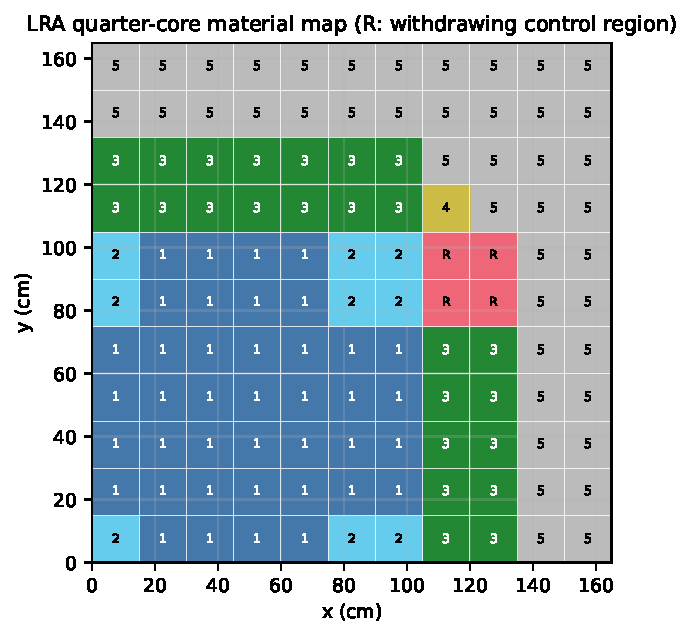
\includegraphics[width=0.62\textwidth]{lra_geometry.pdf}
\caption{Quarter-core material map used by \ndgpu{}. Region R is the four-cell
control region. Performance is measured with four FV cells per assembly edge
(3.75 cm); the ANL convergence study extends to fifteen (1 cm).}
\label{fig:geometry}
\end{figure}

The reference hierarchy matters. The ``Reference'' column in Cherezov et
al.'s Table 6 is explicitly attributed to the fine-mesh finite-difference
ANL-7416/2 dataset of Finnemann. Those values are the primary validation data
in this report. FEMCORE is a secondary calculation using fourth-order
B-spline finite elements and a related adaptive BDF algorithm. Agreement with
FEMCORE alone would not establish agreement with the benchmark.

The source audit also resolved a significant input ambiguity. Cherezov's
printed Table 4 lists both reflector absorptions one decade above the original
ANL/DIF3D data. The corrected values are
$\Sigma_{a1}=6.034\times10^{-4}\ \mathrm{cm}^{-1}$ and
$\Sigma_{a2}=1.911\times10^{-2}\ \mathrm{cm}^{-1}$. Using the printed thermal
value while omitting axial buckling created an accidental rods-in cancellation
and a false rods-out control-worth discrepancy. All calculations here use the
original reflector data and the specified buckling. The Doppler multiplier is
applied to physical fast absorption only, not to the $D_gB_z^2$ leakage term.

There are two feedback-resolution contracts in this report. Cherezov et al.
state that they use one average temperature per finite element and note the
inaccuracy introduced by that approximation. The \ndgpu{} ``assembly'' model
reproduces this choice. The original benchmark equations instead define
$T(t,\mathbf{x})$ and Doppler feedback pointwise. The \ndgpu{} ``cell-local''
model applies those equations on every FV cell and is the spatial-refinement
path used for comparison to the fine-mesh ANL reference. Reported peak
temperature is always the maximum \emph{assembly-average} temperature, matching
the Finnemann/Cherezov comparison field; the hotter maximum computational-cell
temperature is retained in JSON as a separate diagnostic.

\section{Adaptive BDF implementation}

For order $q$, a nonuniform BDF step is written
\begin{equation}
  \sum_{j=0}^{q} a_j u_{n+1-j}=h_n F(u_{n+1}),
\end{equation}
where the coefficients are recomputed from the actual accepted time nodes.
The same recurrence is used for each neutron group and delayed-precursor
family. The coupled LRA temperature correction uses the identical selected
order and time-node history.

The accepted-state vector for error control is
\begin{equation}
 y=\left[\phi_1,\phi_2,C_1,C_2,T\right].
\end{equation}
Given a corrected endpoint $y_c$ and a polynomial endpoint prediction $y_p$,
the normalized defect is
\begin{equation}
 e_h=\left(
 \frac{\sum_i\lVert y_{c,i}-y_{p,i}\rVert_2^2}
      {\sum_i\lVert \mathrm{atol}+\mathrm{rtol}|y_{c,i}|\rVert_2^2}
 \right)^{1/2}.
\end{equation}
A step is accepted when $e_h\le1$. Rejection restores flux, precursor,
temperature, and every BDF history to the last accepted endpoint. The rejected
attempt does not call the external accepted-step hook.

For an accepted order-$q$ step, candidate predictor defects are formed for the
available members of $\{q-1,q,q+1\}$. Each candidate proposes
\begin{equation}
 h_{n+1}(r)=\frac{h_n}{1.25\,(e_r+10^{-6})^{1/(r+1)}},
\end{equation}
bounded to a factor in $[0.2,5]$. The candidate with the largest proposal is
used unless its advantage over retaining $q$ is less than 5\%. Known
discontinuities terminate a step exactly and restart all histories at order
one. This estimator/order comparison reuses the converged endpoint and
therefore adds vector operations but no spatial solve.

The paper-faithful rejection rule retries at $h_n/2$. An optional optimized
rule applies the same defect exponent to a failed attempt, but caps the retry
at $h_n/2$ and floors it at $0.2h_n$. Thus a marginal failure remains as
conservative as the paper rule, while a very large defect can avoid a sequence
of repeated halvings. Rejected endpoint, width, order, and work telemetry make
this overhead directly auditable.

\begin{figure}[ht]
\centering
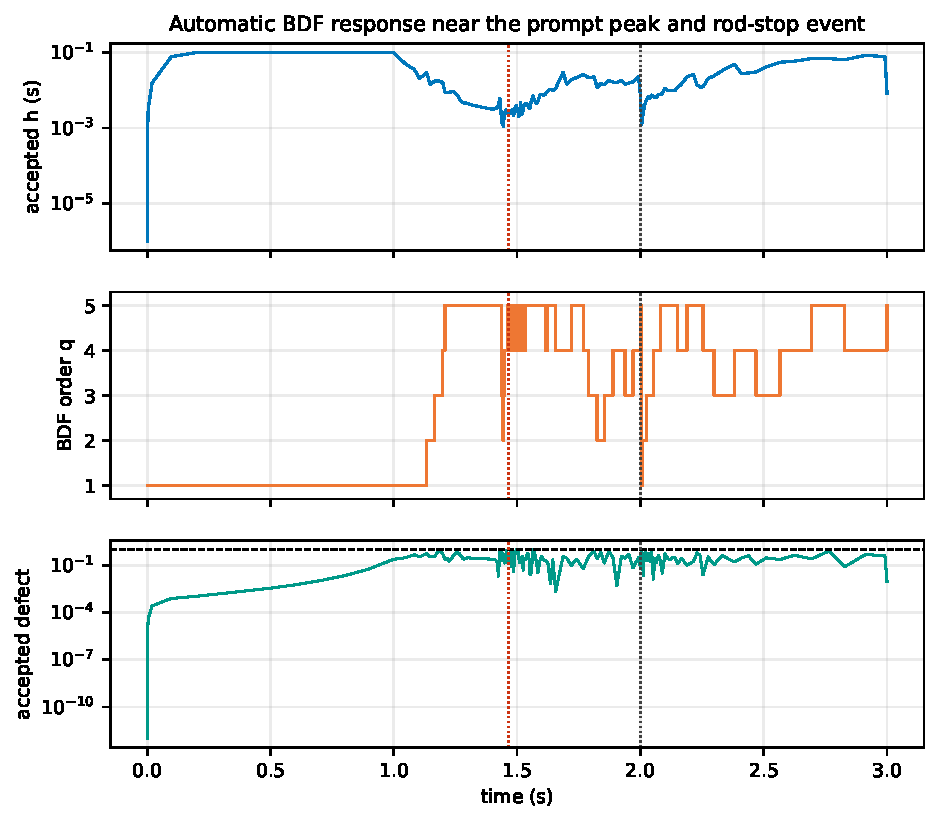
\includegraphics[width=0.94\textwidth]{controller_history.pdf}
\caption{Accepted step width, selected order, and normalized accepted defect
for the practical automatic-BDF run ($\mathrm{RTOL}=10^{-3}$). The red dotted
line is the first power peak; the black dotted line is the 2 s rod-stop event.
The controller contracts to millisecond steps near both rapid changes and
recovers large steps in smooth intervals.}
\label{fig:controller}
\end{figure}

\section{Experimental protocol}

All runs use the corrected LRA definition, fully implicit endpoint constituent
iteration, initial step $10^{-6}$ s, maximum step 0.1 s, and an exact
event/restart at 2 s. The maximum BDF order is five. Performance and tolerance
comparisons use the 3.75 cm mesh; the tight $10^{-6}$ BDF result is their
fixed-model temporal reference. ANL spatial validation uses cell-local feedback
at $\mathrm{RTOL}=10^{-5}$ on 15, 7.5, 3.75, 1.875, and 1 cm meshes. A tight
cell-local 3.75 cm run verifies that $10^{-5}$ contributes only 0.059\% error
to the first peak and negligible error to the remaining reported values.

Three distinctions are maintained throughout:
\begin{enumerate}
\item \textbf{Benchmark accuracy}: difference from the original ANL reference.
\item \textbf{Temporal error}: difference from the tight \ndgpu{} BDF solution
  on the same spatial model.
\item \textbf{Performance}: wall time and solver work at comparable temporal
  error, not at equal step width or equal controller tolerance.
\end{enumerate}

Wall time is measured on one development CPU and is not portable. Accepted
steps, FGMRES operator applications, and preconditioner inner iterations are
reported as architecture-independent work counters. Each history and all
telemetry used in the figures are stored as JSON beside this document.

\section{Accuracy against the original ANL reference}

\subsection{Static endpoints}

\begin{center}
\begin{tabular}{|l|r|r|r|r|}
\hline
Quantity & ANL & \ndgpu{} 3.75 cm & \ndgpu{} 1 cm & FEMCORE \\
\hline
$k_{\mathrm{eff}}$, rods in  & 0.996330 & 0.9962305 & 0.9963254 & 0.996390 \\
$k_{\mathrm{eff}}$, rods out & 1.015460 & 1.0148158 & 1.0153202 & 1.015500 \\
\hline
\end{tabular}
\end{center}

At 1 cm, the rods-in and rods-out differences are $-0.5$ and $-14$ pcm.
The rods-in value also reproduces the archived 1 cm DIF3D result 0.996325.
The endpoint sequence therefore demonstrates ordinary finite-volume mesh
convergence and rules out a missing control worth.

\subsection{Transient observables}

\begin{center}
\small
\begin{tabular}{|l|r|r|r|r|r|}
\hline
Quantity & ANL & Assembly T, 3.75 cm & Cell T, 3.75 cm & Cell T, 1 cm & FEMCORE \\
\hline
First-peak time (s) & 1.436 & 1.46978 & 1.46975 & 1.44432 & 1.439 \\
First-peak power (W/cm$^3$) & 5411 & 5601.56 & 5417.33 & 5397.67 & 5641 \\
Second-peak power (W/cm$^3$) & 784 & 807.20 & 779.03 & 791.99 & 820 \\
Power at 3 s (W/cm$^3$) & 96.2 & 98.8319 & 95.8367 & 98.0318 & 98.7 \\
Mean temperature at 3 s (K) & 1087 & 1084.68 & 1059.80 & 1088.75 & 1122 \\
Peak assembly T at 3 s (K) & 2948 & 2953.16 & 2861.89 & 2946.28 & 3068 \\
\hline
\end{tabular}
\end{center}

The tight assembly-temperature result isolates temporal error but retains
Cherezov's element-wise feedback approximation. Resolving the benchmark's
local feedback changes the 3.75 cm first/second/tail power differences to
$+0.12/-0.63/-0.38\%$. Refining that model to 1 cm gives differences of
$+0.58\%$ in first-peak time, $-0.25\%$ in first-peak power, $+1.02\%$ in
second-peak power, and $+1.90\%$ in tail power. Mean and peak assembly
temperature differ by only $+0.16\%$ and $-0.06\%$. FEMCORE's largest Table 6
difference is 4.59\% at the second peak.

\begin{figure}[ht]
\centering
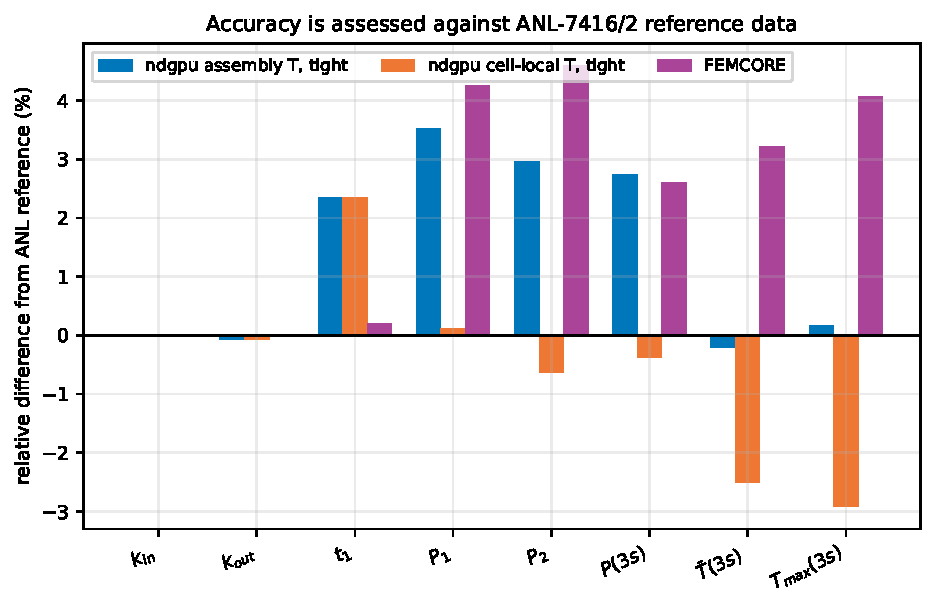
\includegraphics[width=0.94\textwidth]{anl_accuracy.pdf}
\caption{Feedback resolution at fixed 3.75 cm mesh. Cell-local feedback moves
all three power values substantially closer to ANL; assembly-averaged feedback
remains the appropriate reproduction of Cherezov's stated approximation.
FEMCORE is secondary, not the reference baseline.}
\label{fig:accuracy}
\end{figure}

Figure~\ref{fig:power} places the original point references on the computed
histories. The practical assembly-temperature $10^{-3}$ BDF first peak nearly
equals ANL by temporal/spatial error cancellation; the converged 1 cm
cell-local history instead approaches the reference consistently across the
full reporting set.

\begin{figure}[ht]
\centering
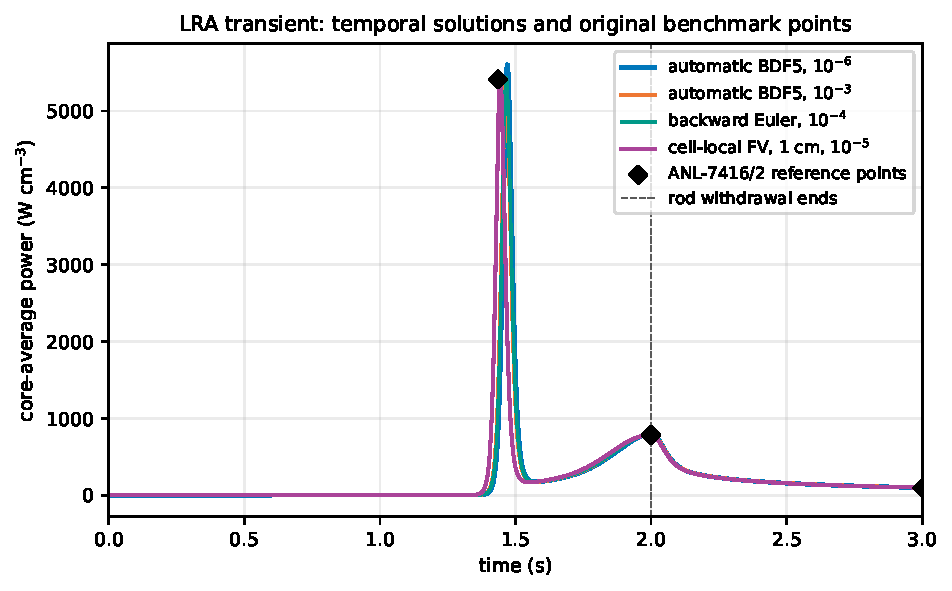
\includegraphics[width=0.96\textwidth]{power_history.pdf}
\caption{Complete accepted power histories with the three original ANL point
references. The black line marks the end of linear control withdrawal. The
1 cm cell-local curve is the spatially refined validation result; the other
curves support the fixed-mesh performance comparison.}
\label{fig:power}
\end{figure}

\subsection{Spatial convergence of the benchmark model}

\begin{center}
\small
\begin{tabular}{|r|r|r|r|r|r|r|}
\hline
Cell (cm) & $t_1$ & $P_1$ & $P_2$ & $P(3s)$ & $\bar T(3s)$ & $T_{max}(3s)$ \\
\hline
15 & $-9.31\pct$ & $+10.38\pct$ & $+31.18\pct$ & $+17.25\pct$ & $+24.57\pct$ & $+50.54\pct$ \\
7.5 & $+1.04\pct$ & $+1.65\pct$ & $+3.68\pct$ & $+1.39\pct$ & $+0.45\pct$ & $+3.56\pct$ \\
3.75 & $+2.36\pct$ & $+0.06\pct$ & $-0.63\pct$ & $-0.38\pct$ & $-2.50\pct$ & $-2.92\pct$ \\
1.875 & $+1.25\pct$ & $+0.20\pct$ & $+0.46\pct$ & $+1.10\pct$ & $-0.81\pct$ & $-1.22\pct$ \\
1 & $+0.58\pct$ & $-0.25\pct$ & $+1.02\pct$ & $+1.90\pct$ & $+0.16\pct$ & $-0.06\pct$ \\
\hline
\end{tabular}
\end{center}

The convergence is not monotone for every scalar---material interfaces,
peak sampling, and feedback interact---but the envelope contracts decisively.
At 1 cm all six transient values lie within 1.90\% and both eigenvalues within
14 pcm. The hottest 1 cm computational cell reaches 3329 K; it is not compared
to the 2948 K assembly-distribution reference and is stored separately.

\begin{figure}[ht]
\centering
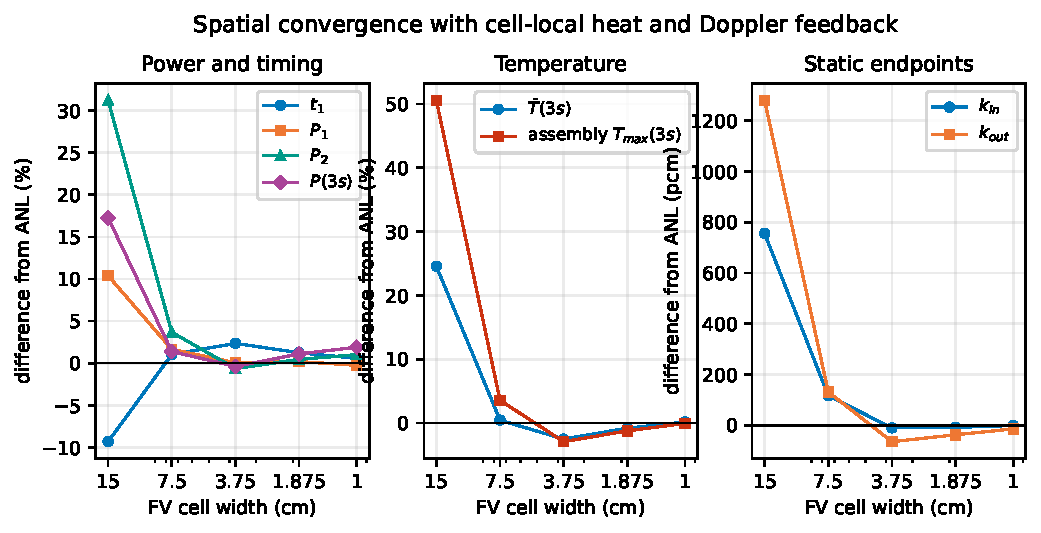
\includegraphics[width=0.98\textwidth]{spatial_convergence.pdf}
\caption{Signed spatial convergence against ANL using cell-local heat and
Doppler feedback. Peak temperature denotes the maximum assembly average.}
\label{fig:spatial}
\end{figure}

\section{Temporal convergence at fixed spatial model}

\begin{center}
\small
\begin{tabular}{|r|r|r|r|r|r|r|}
\hline
RTOL & Acc./rej. & Inner its. & $t_1$ (s) & $P_1$ & $P_2$ & $P(3\,s)$ \\
\hline
$10^{-3}$ & 199/22 & 301861 & 1.46589 & 5409.93 & 806.42 & 98.82496 \\
$10^{-4}$ & 284/22 & 294134 & 1.46818 & 5563.33 & 807.08 & 98.82945 \\
$10^{-5}$ & 414/29 & 341182 & 1.46997 & 5599.09 & 807.19 & 98.83172 \\
$10^{-6}$ & 605/28 & 421475 & 1.46978 & 5601.56 & 807.20 & 98.83190 \\
\hline
\end{tabular}
\end{center}

The first prompt peak controls the tolerance requirement. Relative to the
$10^{-6}$ temporal result, its error is $-3.42\%$, $-0.68\%$, and $-0.044\%$
at $10^{-3}$, $10^{-4}$, and $10^{-5}$. The second peak, tail power, and final
temperatures converge much sooner. The slightly smaller inner count at
$10^{-4}$ than $10^{-3}$ is real: the looser run attempts more aggressive
width/order changes and pays more rejected and constituent work.

The table uses the assembly-temperature track so that only temporal controls
change. The cell-local check gives the same conclusion: tightening from
$10^{-5}$ to $10^{-6}$ changes $P_1$ from 5414.13 to 5417.33 W/cm$^3$
(0.059\%), while $P_2$, tail power, and both final temperatures change by less
than 0.002\%. Smaller steps converge the semi-discrete model; they cannot by
themselves remove spatial or feedback-resolution error.

\begin{figure}[ht]
\centering
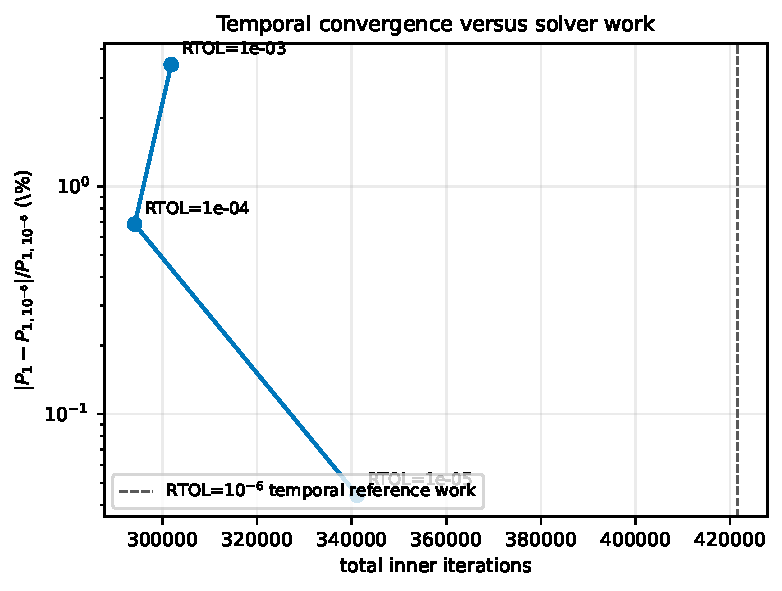
\includegraphics[width=0.72\textwidth]{tolerance_tradeoff.pdf}
\caption{First-peak temporal convergence versus total inner iterations. The
dashed line records the cost of the tight temporal reference; it is not plotted
as a fictitious nonzero error point.}
\label{fig:tolerance}
\end{figure}

\section{Performance of adaptive BDF}

At the paper's $10^{-5}$ controls, automatic order gives 414 accepted and 29
rejected steps, compared with 461/21 when the maximum available order is held.
The histories agree at reporting precision. Automatic selection cuts accepted
steps by 10.2\%, FGMRES applications by 3.4\%, inner iterations by 3.2\%, and
measured time by 4.7\%. The accepted count is close to the 399 regular steps
reported for fourth-order FEMCORE; rejection counts are not directly
equivalent because the state norms and spatial discretizations differ.

The main performance comparison uses the benchmark-faithful cell-local model
and matches temporal accuracy. Relative to its tight BDF result, practical
automatic BDF5 at $10^{-3}$ has $-3.11\%$ first-peak error. Backward Euler
requires $10^{-4}$ to reach a comparable $-2.92\%$ error. Their first-peak-time
errors are $-0.35\%$ and $-0.27\%$; tail and temperature errors are smaller.

\begin{center}
\small
\begin{tabular}{|l|r|r|r|r|r|r|}
\hline
Method & RTOL & Acc./rej. & FGMRES & Inner & CPU (s) & $P_1$ error \\
\hline
Automatic BDF5 & $10^{-3}$ & 201/30 & 13129 & 315381 & 27.54 & $-3.11\pct$ \\
Backward Euler & $10^{-4}$ & 3180/19 & 66671 & 1512769 & 140.54 & $-2.92\pct$ \\
\hline
BE/BDF ratio & --- & 15.82x & 5.08x & 4.80x & 5.10x & comparable \\
\hline
\end{tabular}
\end{center}

\begin{figure}[ht]
\centering
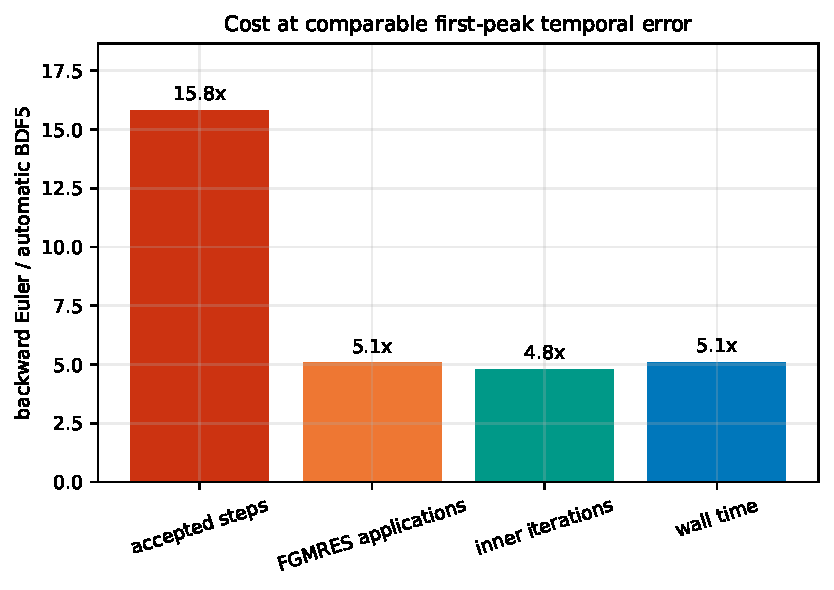
\includegraphics[width=0.76\textwidth]{matched_cost.pdf}
\caption{Backward-Euler cost divided by automatic-BDF5 cost at comparable
first-peak temporal error. Work-counter ratios are more portable than the
single-host wall-time ratio.}
\label{fig:cost}
\end{figure}

This matched result is materially different from comparing methods at equal
$h$ or equal RTOL. Equal step widths strongly over-damp backward Euler near the
prompt peak. Equal controller tolerances are also inappropriate because the
predictor/corrector defect has a different order and error constant for each
method.

\subsection{Rejected-step overhead}

At the practical $10^{-3}$ tolerance, the optional error-scaled retry with a
0.5 cap retains 201 accepted steps but reduces rejected steps from 30 to 25.
The following CPU values are medians of three sequential samples; deterministic
work counters are identical across repetitions.

\begin{center}
\small
\begin{tabular}{|l|r|r|r|r|r|}
\hline
Rejection policy & Acc./rej. & FGMRES & Rej. FGMRES & Inner & CPU (s) \\
\hline
Factor two & 201/30 & 13129 & 2523 & 315381 & 26.876 \\
Error-scaled, cap 0.5 & 201/25 & 12395 & 2144 & 297831 & 25.494 \\
\hline
Reduction & --- & 5.59\% & 15.0\% & 5.56\% & 5.14\% \\
\hline
\end{tabular}
\end{center}

The optimized rule removes the two repeated-rejection streaks observed with
factor-two control. Its first peak moves from 5248.71 to
5313.11 W cm$^{-3}$, closer to the ANL value of 5411 W cm$^{-3}$; tail and
temperature observables change by at most 0.043\%. At $10^{-5}$ the policies
are work-neutral (14159 versus 14160 FGMRES applications), and first-peak time
and power are identical at stored precision. A less conservative 0.8 cap was
rejected: it induced a BDF1 reject/accept oscillation and increased the tight
run to 623 accepted and 140 rejected steps. Error-scaled rejection therefore
remains opt-in pending the HP-MR stability progression.

\subsection{CPU comparison with Cherezov et al.}

Cherezov et al.'s Tables 7--8 provide both a BDF work row and CPU time by FEM
order. Their fourth-order accuracy calculation is the closest published
spatial-size comparison to the 3.75 cm FV case: 2025 scalar degrees of freedom
versus 1936 FV cells. Both use $\mathrm{RTOL}=10^{-5}$ and automatic BDF up to
order five.

\begin{center}
\small
\begin{tabular}{|l|r|r|r|r|r|}
\hline
Calculation & Spatial size & Acc./rej. & CPU (s) & Max. ANL diff. & Host \\
\hline
\ndgpu{} FV, 3.75 cm & 1936 cells & 410/27 & 28.62 & 2.92\% & i5-1145G7 \\
FEMCORE, FEM order 4 & 2025 DOF & 399/7 & 29.1 & 4.59\% & not reported \\
\ndgpu{} FV, 1 cm & 27225 cells & 391/29 & 614.50 & 1.90\% & i5-1145G7 \\
\hline
\end{tabular}
\end{center}

The 28.62 s and 29.1 s values are remarkably close, but they are \emph{not} a
cross-code speedup: FEMCORE's processor, thread configuration, compiler, and
timing scope are not stated. The accepted-step comparison is more portable and
also close. Solver iteration columns are not equated because FEMCORE counts
block-GS/Anderson and ILU-CG operations, whereas \ndgpu{} counts monolithic
FGMRES applications and preconditioner PCG iterations.

For completeness, the published FEMCORE CPU ladder for FEM orders 1--8 is
1.4, 4.7, 12.2, 29.1, 62.2, 121.7, 237.0, and 438.1 s. Figure~\ref{fig:cpu}
plots those raw times with the two \ndgpu{} measurements. It communicates
computational scale, not normalized throughput.

\begin{figure}[ht]
\centering
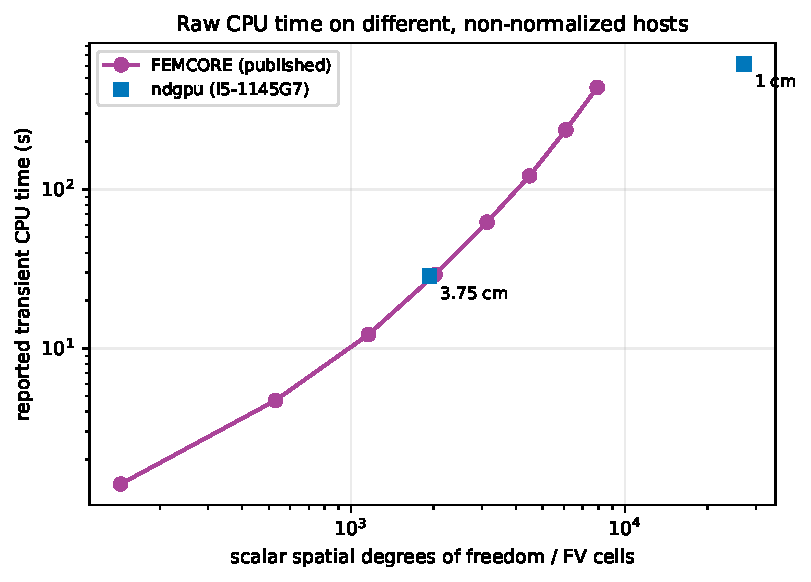
\includegraphics[width=0.72\textwidth]{cherezov_cpu.pdf}
\caption{Published FEMCORE and measured \ndgpu{} transient CPU times. The
hosts differ and FEMCORE's hardware is not disclosed; no cross-code speedup is
formed.}
\label{fig:cpu}
\end{figure}

\subsection{Transferability of the LRA speedup}

The fivefold LRA result is not a universal BDF-over-BE factor. A subsequent
11-group HP-MR slow-drum test at matched \texttt{RTOL=$10^{-3}$} gives 29/8
accepted/rejected steps for adaptive BE and 29/9 for automatic BDF5. BDF uses
23 order-one and six order-two steps; its 14.29 s coupled time is 5.3\% above
BE's 13.58 s, while its maximum power error is modestly smaller (0.0208\%
versus 0.0278\%). The same conclusion holds in an accelerated-thermal
feedback stress test.

The difference is temporal rather than spatial-solver throughput. LRA's sharp
prompt and rod-stop peaks require 3180 BE steps for the accuracy reached by 201
BDF steps. The mild HP-MR maneuver is nearly linear between control knots, so
the full-state selector correctly remains at orders one and two and adaptive
BE chooses essentially the same widths. Comparisons against a deliberately
fine 64-step BE reference still show a 1.5--2.0x cost reduction, but that is an
adaptive-versus-reference result, not evidence that high-order BDF beats BE at
matched error.

A subsequent 3-D GPU gate confirms the same mechanism on a Tesla T4. The
11-group refinement-2 core with ten axial layers has 145,200 active flux
unknowns. Against a 32-step fixed-BE reference, adaptive BE takes 24 accepted
and seven rejected steps, while automatic BDF5 takes 22 accepted and nine
rejected steps. BDF remains mostly low order (15 BDF1 and seven BDF2 steps),
but has the smaller maximum power error (0.0260\% versus 0.0301\%) and a
fivefold smaller final normalized flux-shape error.

Three interleaved short solves resolve the GPU preconditioner choice. Plain
tolerance-based group PCG has a 2.310 s median. Adding energy Anderson raises
it to 2.620 s and is rejected; four reduction-free polynomial sweeps with
depth-one Anderson take 2.098 s, a 1.101x gain over plain PCG. Two complete
runs with that polynomial configuration put the matched BDF/BE speed ratio at
0.946x and 0.902x: BDF is consistently 5.7--10.9\% slower. In the latest run,
BDF saves 88 outer applications on accepted attempts, but spends 286 extra on
rejected attempts, for 2260 total versus 2062 for BE. The implementation gates
pass: energy-group batching is active, persistent FGMRES storage is 61.27 MiB,
and the latest one-transfer error norm and fused history predictor are 1.569x
and 1.388x faster. The next acceleration target is therefore rejected-attempt
Krylov work, not adaptive bookkeeping or another energy correction. Reference
doubling and the production-size GPU case remain required.

\clearpage

\section{Limitations and interpretation}

\begin{itemize}
\item \textbf{Spatial method.} \ndgpu{} uses cell-centred finite volume;
  FEMCORE uses high-order B-spline FEM. The five-mesh ladder demonstrates the
  finite-volume envelope rather than assuming equivalence by nominal DOF.
\item \textbf{Sparse reference history.} The original comparison contract
  provides peak and endpoint values rather than a digitized, uncertainty-rated
  continuous trace. The plotted black diamonds are those point references;
  lines between them are not invented.
\item \textbf{Observable definition.} ANL/Cherezov spatial temperature values
  are assembly averaged. A cell-local simulation also has a hotter cell
  maximum; reporting it as the benchmark peak would mix observables.
\item \textbf{Error cancellation.} Loose-tolerance and intermediate-mesh
  agreement can be fortuitous. Accuracy claims use a temporal check plus the
  full spatial sequence, not the closest isolated scalar.
\item \textbf{Timing portability.} The within-host 5.08x FGMRES and 4.80x
  inner-work ratios are stronger evidence than seconds. Cherezov's CPU is
  unknown, so its raw time is not used to claim a speedup. The Tesla T4 quick
  gate is a same-device comparison. Repeated polynomial-preconditioned runs
  show BDF 5.7--10.9\% slower than matched BE on the mild HP-MR trajectory;
  this is reported as a case-specific negative result, not a universal ratio.
\item \textbf{Controller overhead.} Candidate-order defects require no spatial
  solve. The conservative error-scaled retry reduces practical-tolerance LRA
  rejection work, but the paper-control calculation still has more rejections
  than FEMCORE and uses a different state norm.
\end{itemize}

\section{Conclusion}

The corrected LRA model provides a demanding and useful validation case for
adaptive time integration: it combines a prompt-supercritical peak, delayed
neutrons, a moving control perturbation, a feedback-driven decline, a second
peak at the rod-stop event, and strongly nonuniform useful time scales. The new
\ndgpu{} BDF path resolves that history without instability, respects the full
coupled-state error test and event rollback contract, and converges toward the
original ANL data as the cell-local model is refined. At 1 cm all six transient
checks are within 1.90\%, temperature checks within 0.17\%, and static endpoints
within 14 pcm.

Performance is not inferred from equal time steps. At matched first-peak
temporal accuracy, automatic BDF5 reduces portable linear-solver work by about
a factor of five and measured CPU time by a factor of 5.10 relative to adaptive
backward Euler. At paper controls and comparable spatial size, the raw \ndgpu{}
and FEMCORE times are 28.62 and 29.1 s; the unknown FEMCORE hardware precludes
a cross-code speedup claim. The combined accuracy and within-host performance
evidence supports carrying the controller into the staged HP-MR transient
cases. Error-scaled rejection provides a further 5.6\% deterministic work
reduction at practical tolerance, while factor-two rejection remains the
paper-faithful default. The 3-D T4 quick gate preserves accuracy and validates
the optimized GPU path, including a 1.101x repeated-median gain from its
reduction-free polynomial preconditioner. It nevertheless shows no matched
BDF-over-BE speedup on mild HP-MR motion because rejected BDF attempts dominate
the saved accepted-step work. Adaptive BDF stays opt-in until reference
convergence and production-scale HP-MR gates are complete.

\section*{Reproducibility}

From the repository root, the structured aggregate benchmark is
\begin{verbatim}
PYTHONPATH=. python examples/lra2d_bdf_tolerance_benchmark.py --refine 4
\end{verbatim}
The fine-mesh accuracy endpoint is reproduced with
\begin{verbatim}
PYTHONPATH=. python examples/lra2d_bdf_benchmark.py --refine 15 \
  --dt 1e-6 --order 5 --implicit-feedback --thermal-zones cell \
  --adaptive-rtol 1e-5 --automatic-order --include-static-endpoints
\end{verbatim}
The complete-history JSON files were produced with
\code{examples/lra2d\_bdf\_benchmark.py --include-history --output ...}.
Run \code{make} in this report directory to regenerate figures and PDF from
the stored data. The complete repository regression at this checkpoint is 575
passed, 5 skipped, and 13 deselected; the focused LRA/BDF subset is 82 passed.

\begin{thebibliography}{9}
\bibitem{finnemann1977}
H. Finnemann, \emph{Argonne Code Center: Benchmark Problem Book, Volume 2},
Argonne National Laboratory, 1977. DOI: \url{https://doi.org/10.2172/12030251}.

\bibitem{cherezov2025}
A. Cherezov, A. Vasiliev, and H. Ferroukhi,
``Application of Backward Differential Formula and Anderson's method for
multigroup diffusion transient equation,'' \emph{Annals of Nuclear Energy},
210, 110837, 2025. DOI:
\url{https://doi.org/10.1016/j.anucene.2024.110837}.

\bibitem{dif3darchive}
Core Physics LLC, ``LRA benchmark: archived fine-mesh DIF3D input and
results,'' \url{https://corephysics.com/benchmarks/dif3d_lra.txt}, accessed
18 August 2026.
\end{thebibliography}

\end{document}
